\documentclass[acmsmall,nonacm]{acmart}

\setcopyright{none}
\settopmatter{printacmref=false}
\renewcommand\footnotetextcopyrightpermission[1]{}
\pagestyle{plain}

\usepackage[UTF8, scheme=plain, punct=plain, zihao=false]{ctex}
\usepackage{xcolor}
\usepackage{fontspec}
\usepackage{natbib}
\usepackage{xeCJK}
\usepackage{graphicx}
\graphicspath{{images/}} 
\setCJKsansfont{PingFang SC}

\newcommand{\makelabreportcover}{
  \clearpage
  \thispagestyle{empty}
  \sffamily 
  
  % University logo
    \begin{center}
  
\includegraphics[height=2cm]{logo.png}
  \end{center}
  
  \vspace{1.5cm}
  
  % Course title
  \begin{center}
  {\fontsize{22}{30}\selectfont\bfseries Internet of Things Engineering Practices\par}
  
  \vspace{1cm}
  
  {\fontsize{26}{32}\selectfont\bfseries Lab Report\par}
  \end{center}
  
  \vfill
  
  % Experiment information
  \begin{center}
  \Large\bfseries
  
  \vspace{1cm}
  
  \begin{tabular}{@{}c@{}}
    Experiment Title \\[0.8em]
    {\fontsize{18}{22}\selectfont RFID Basic Operation}
  \end{tabular}
  
  \vspace{1cm}
  
  % Group Number
  \begin{tabular}{@{}c@{}}
    Group Number \\[0.8em]
    {\fontsize{12}{16}\selectfont No.~1}
  \end{tabular}
  
  \vspace{1cm}
  
  % Group Members
  \begin{tabular}{@{}c@{}}
    Group Members \\[0.5em]
  \end{tabular}
    
  \normalsize
  \renewcommand{\arraystretch}{1.6}%
  \begin{tabular}{@{}l@{\hspace{2em}}l@{\hspace{2em}}l@{}}
    金临 & JIN, Lin & 2022210000 \\
    银临 & XIANG, Rachel & 2022211111 \\
    铜临 & TONG, Lin & 2022212222
  \end{tabular}
  
  \vspace{1cm}
  
  \begin{tabular}{@{}c@{}}
  Date \\[0.1em]
  {\normalsize \today}
\end{tabular}
  
  \end{center}
  
  \clearpage
  \setcounter{page}{1}%
}

%===========================================
% Document begins
%===========================================

\begin{document}

% Set a minimal title to avoid errors
\title{RFID Basic Operation}

% Generate custom cover page
\makelabreportcover

%===========================================
% Main content begins directly
%===========================================

\section{Experiment Objective}

\begin{enumerate}
  \item Understanding of the composition, structure and function of the RFID system.
  \item Learning to set up the SDK of RFID system and connecting the reader-transponder module to RFID software. Understanding of the working mode of RFID system.
  \item Analyzing the data formats of EPC tag.
\end{enumerate}

\section{Experiment Procedure}

\textbf{Step 1.} Read the \textit{XinTaiRadio\_User\_Guide} handbook and learn how to install \textit{XinTaiRadio} software.

\textbf{Step 2.} Connect some of the RFID modules, antenna, power etc to the computer as shown in figure \ref{img:demo}.

\begin{figure}[h]
  \centering
  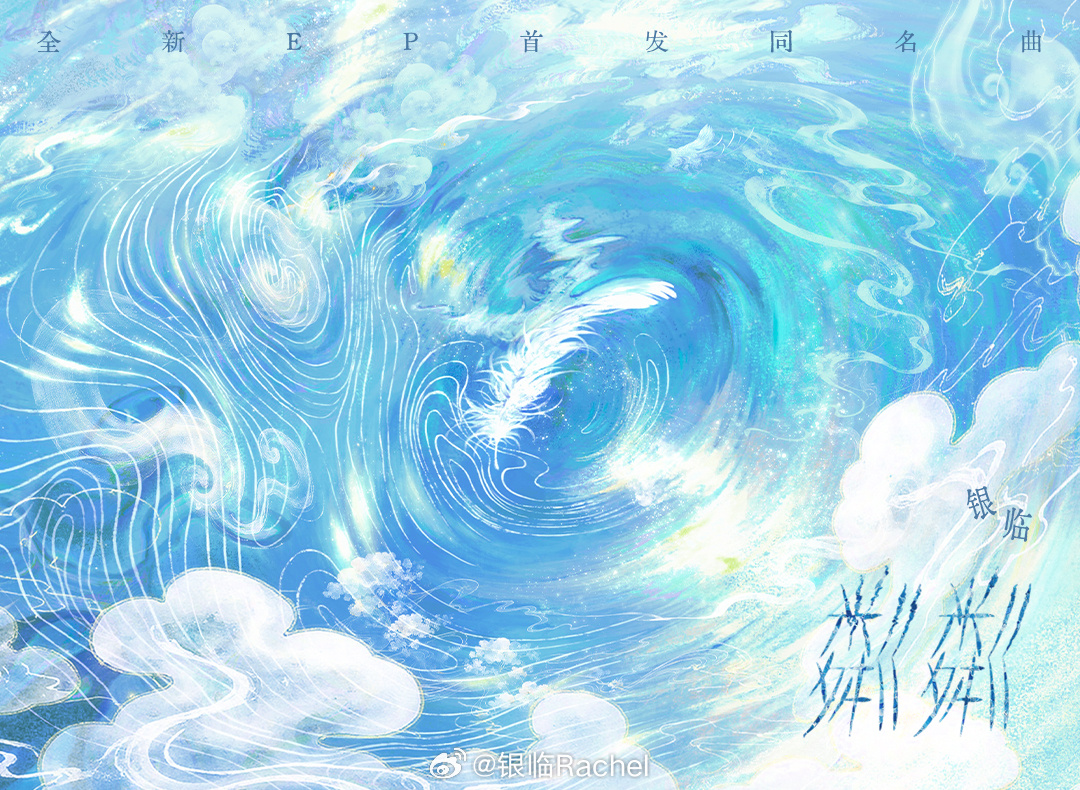
\includegraphics[width=0.8\linewidth]{demo}
  \caption{Demo Picture in \LaTeX{}}
  \Description{demo image}
  \label{img:demo}
\end{figure}

\textbf{Step 3.} When all of these components come together, use \textit{XinTaiRadio} software to do inventory, reading and writing to the tags.

RFID technology has been widely adopted in various applications~\cite{want2006introduction}. The EPC global standard provides a framework for RFID implementations~\cite{epcglobal2008epc}.

\section{Experiment Results}

In this section, describe your experimental results and observations.

\subsection{RFID Tag Reading}

Describe the results of reading RFID tags, including EPC codes and other relevant data. Modern RFID systems operate at different frequencies, each with specific advantages, as shown in table \ref{tab:rfid_results}.

\begin{table}[h]
  \centering
  \caption{RFID Tag Reading Results}
  \label{tab:rfid_results}
  \begin{tabular}{lcc}
    \toprule
    \textbf{Tag ID} & \textbf{Distance (cm)} & \textbf{Signal Strength (dBm)} \\
    \midrule
    E200001234567890 & 50 & -45 \\
    E200001234567891 & 75 & -52 \\
    E200001234567892 & 100 & -58 \\
    E200001234567893 & 125 & -65 \\
    E200001234567894 & 150 & -72 \\
    \bottomrule
  \end{tabular}
\end{table}

\subsection{Data Analysis}

Analyze the format and structure of the data obtained from the RFID tags. Security considerations in RFID systems are critical~\cite{juels2006rfid}.

\section{Discussion}

Discuss the implications of your findings and any challenges encountered during the experiment. Recent advances in IoT have expanded RFID applications~\cite{atzori2010internet}.

\section{Conclusion}

Summarize the key findings and what you learned from this experiment. This experiment demonstrated the basic operation of RFID systems and provided hands-on experience with RFID reader-transponder modules.

\bibliographystyle{unsrt} 
\bibliography{references}

\end{document}